\section{Kinetic Energy of a Vortex Structure}

The first contribution to the Lagrangian in the Vortex Æther Model (VAM) arises from the classical kinetic energy of a fluid with local swirl velocity $\vec{v}$ and æther density $\rho_{\ae}$:
\[
    \mathcal{L}_\text{kin} = \frac{1}{2} \rho_{\ae} |\vec{v}|^2
\]

We consider a stable knotted vortex structure in which the core velocity reaches a characteristic maximum given by the swirl speed $C_e$, intrinsic to the vortex's topological character:
\[
    |\vec{v}| \approx C_e \quad \Rightarrow \quad \mathcal{L}_\text{kin} \sim \frac{1}{2} \rho_{\ae} C_e^2
\]

Since the vortex core has a typical radius $r_c$, the total kinetic energy of a single vortex knot can be approximated by integrating over its core volume:
\[
    E_\text{kin} \approx \frac{1}{2} \rho_{\ae} C_e^2 \cdot \frac{4}{3}\pi r_c^3
\]

This leads to a natural definition of an effective inertial mass for the vortex:
\[
    m_\text{eff} = \rho_{\ae} \cdot \frac{4}{3}\pi r_c^3
    \quad \Rightarrow \quad E = \frac{1}{2} m_\text{eff} C_e^2
\]

In VAM, this expression replaces the conventional notion of inertial mass. It ties the particle’s inertial properties directly to the geometric and dynamical features of its knotted vortex configuration—namely its core radius $r_c$ and swirl speed $C_e$.

\subsection*{Circulation and Inertia}

The circulation around the vortex core is defined as:
\[
    \Gamma = \oint_{\partial S} \vec{v} \cdot d\vec{\ell} = 2\pi r_c C_e
\]

\begin{figure}[h!]
\centering
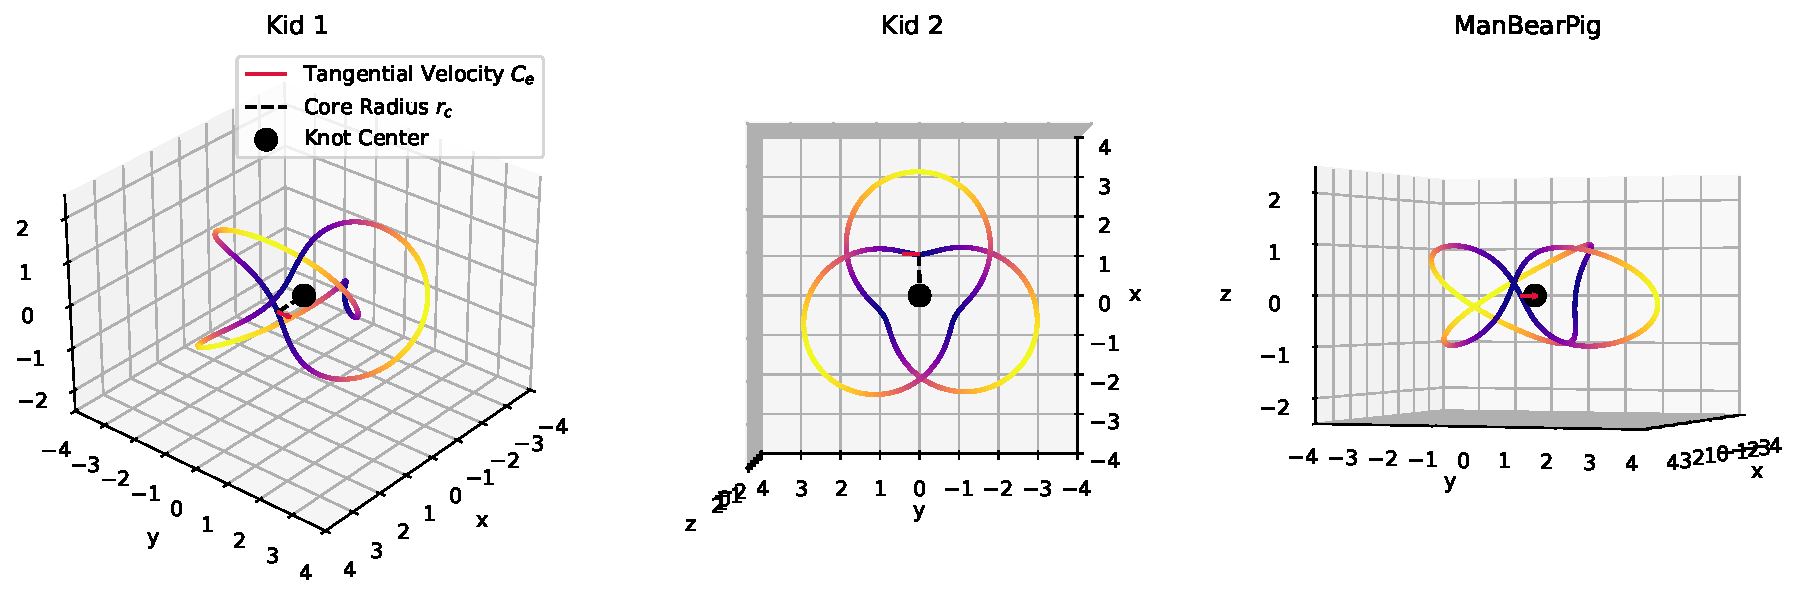
\includegraphics[width=0.95\textwidth]{vortex_knot_diagram}
\caption{Annotation of core radius $r_c$ and swirl direction $C_e$.}
\end{figure}

In an ideal æther, circulation $\Gamma$ is a conserved quantity. As a result, any change in core radius $r_c$ must be accompanied by a compensating change in $C_e$. This coupling underlies the inertial resistance to deformation and reflects a geometric form of inertia. The derived effective mass becomes a function of circulation and vortex rigidity:
\[
    m \propto \frac{\Gamma^2}{r_c C_e^2} = \text{const.}
\]

This kinetic formulation provides the physical basis for mass generation within the VAM framework and aligns with the Lagrangian structure developed in Section~\ref{sec:lagrangian_vam}.
